\normalsize
\section{Solitary Wave Test}
As mentioned by Miles \cite{Miles1980} and Ramaswamy \cite{Ramaswamy1990}, the observation of a solitary wave traveling in a uniform-depth rectangular channel can be dated back to 1834 by John Scott Russell. The solitary wave was idealized as single wave traveling with constant shape and without disturbances in the surrounding water level, i.e., the traveling single permanent wave is neither followed nor preceded by another elevation or depression wave.
Laitone's analytical approximation for such solitary wave \cite{Laitone1960, Jankowski1999} is used to compare the numerical results.
\begin{equation}
\eta = d + Hsech^2[\sqrt{\frac{3H}{4d^3}}(x-ct)]
\end{equation}
\begin{equation}
u = \sqrt{gd}\frac{H}{d}sech^2[\sqrt{\frac{3H}{4d^3}}(x-ct)]
\end{equation}
\begin{equation}
w = \sqrt{3gd}(\frac{H}{d})^{3/2}\ \frac{z}{d} \
sech^2[\sqrt{\frac{3H}{4d^3}}(x-ct)] \
tanh[\sqrt{\frac{3H}{4d^3}}(x-ct)]
\end{equation}
where $d$ is the undisturbed water depth, $H$ is the solitary wave amplitude, $\eta$ is the water level distribution, and the celerity $c$ of the wave is:
\begin{equation}
c=\sqrt{g(H+d)}
\end{equation}

The two-dimensional channel length is 1000$(m)$ and discretized with $\Delta x = 2 (m)$ and $\Delta z = 0.5 (m)$. The undisturbed water depth is $10 (m)$ and the solitary wave amplitude is set to $1 (m)$. The time step is tested with $\Delta t = 0.5(sec)$ and the diffusion coefficient is set to zero.
The inflow boundary condition is specified from the analytical solution at $t=0$ with the wave crest positioned at $x=-150 (m)$. The outflow boundary uses the Sommerfeld open boundary condition \cite{Sommerfeld1949} with the phase speed specified the same as the solitary wave celerity $c=\sqrt{g(H+d)}$. The similarity between the numerical results and the analytical solutions can be seen in Figure \ref{fig:SoliWav-LongCh-Anal-Num-Compar}, where the numerical results and the analytical solutions are plotted at $ t=20(s), 45(s), 70(s)$, and $95(s)$.

\begin{figure}[htbp]
\hspace{0.5in}
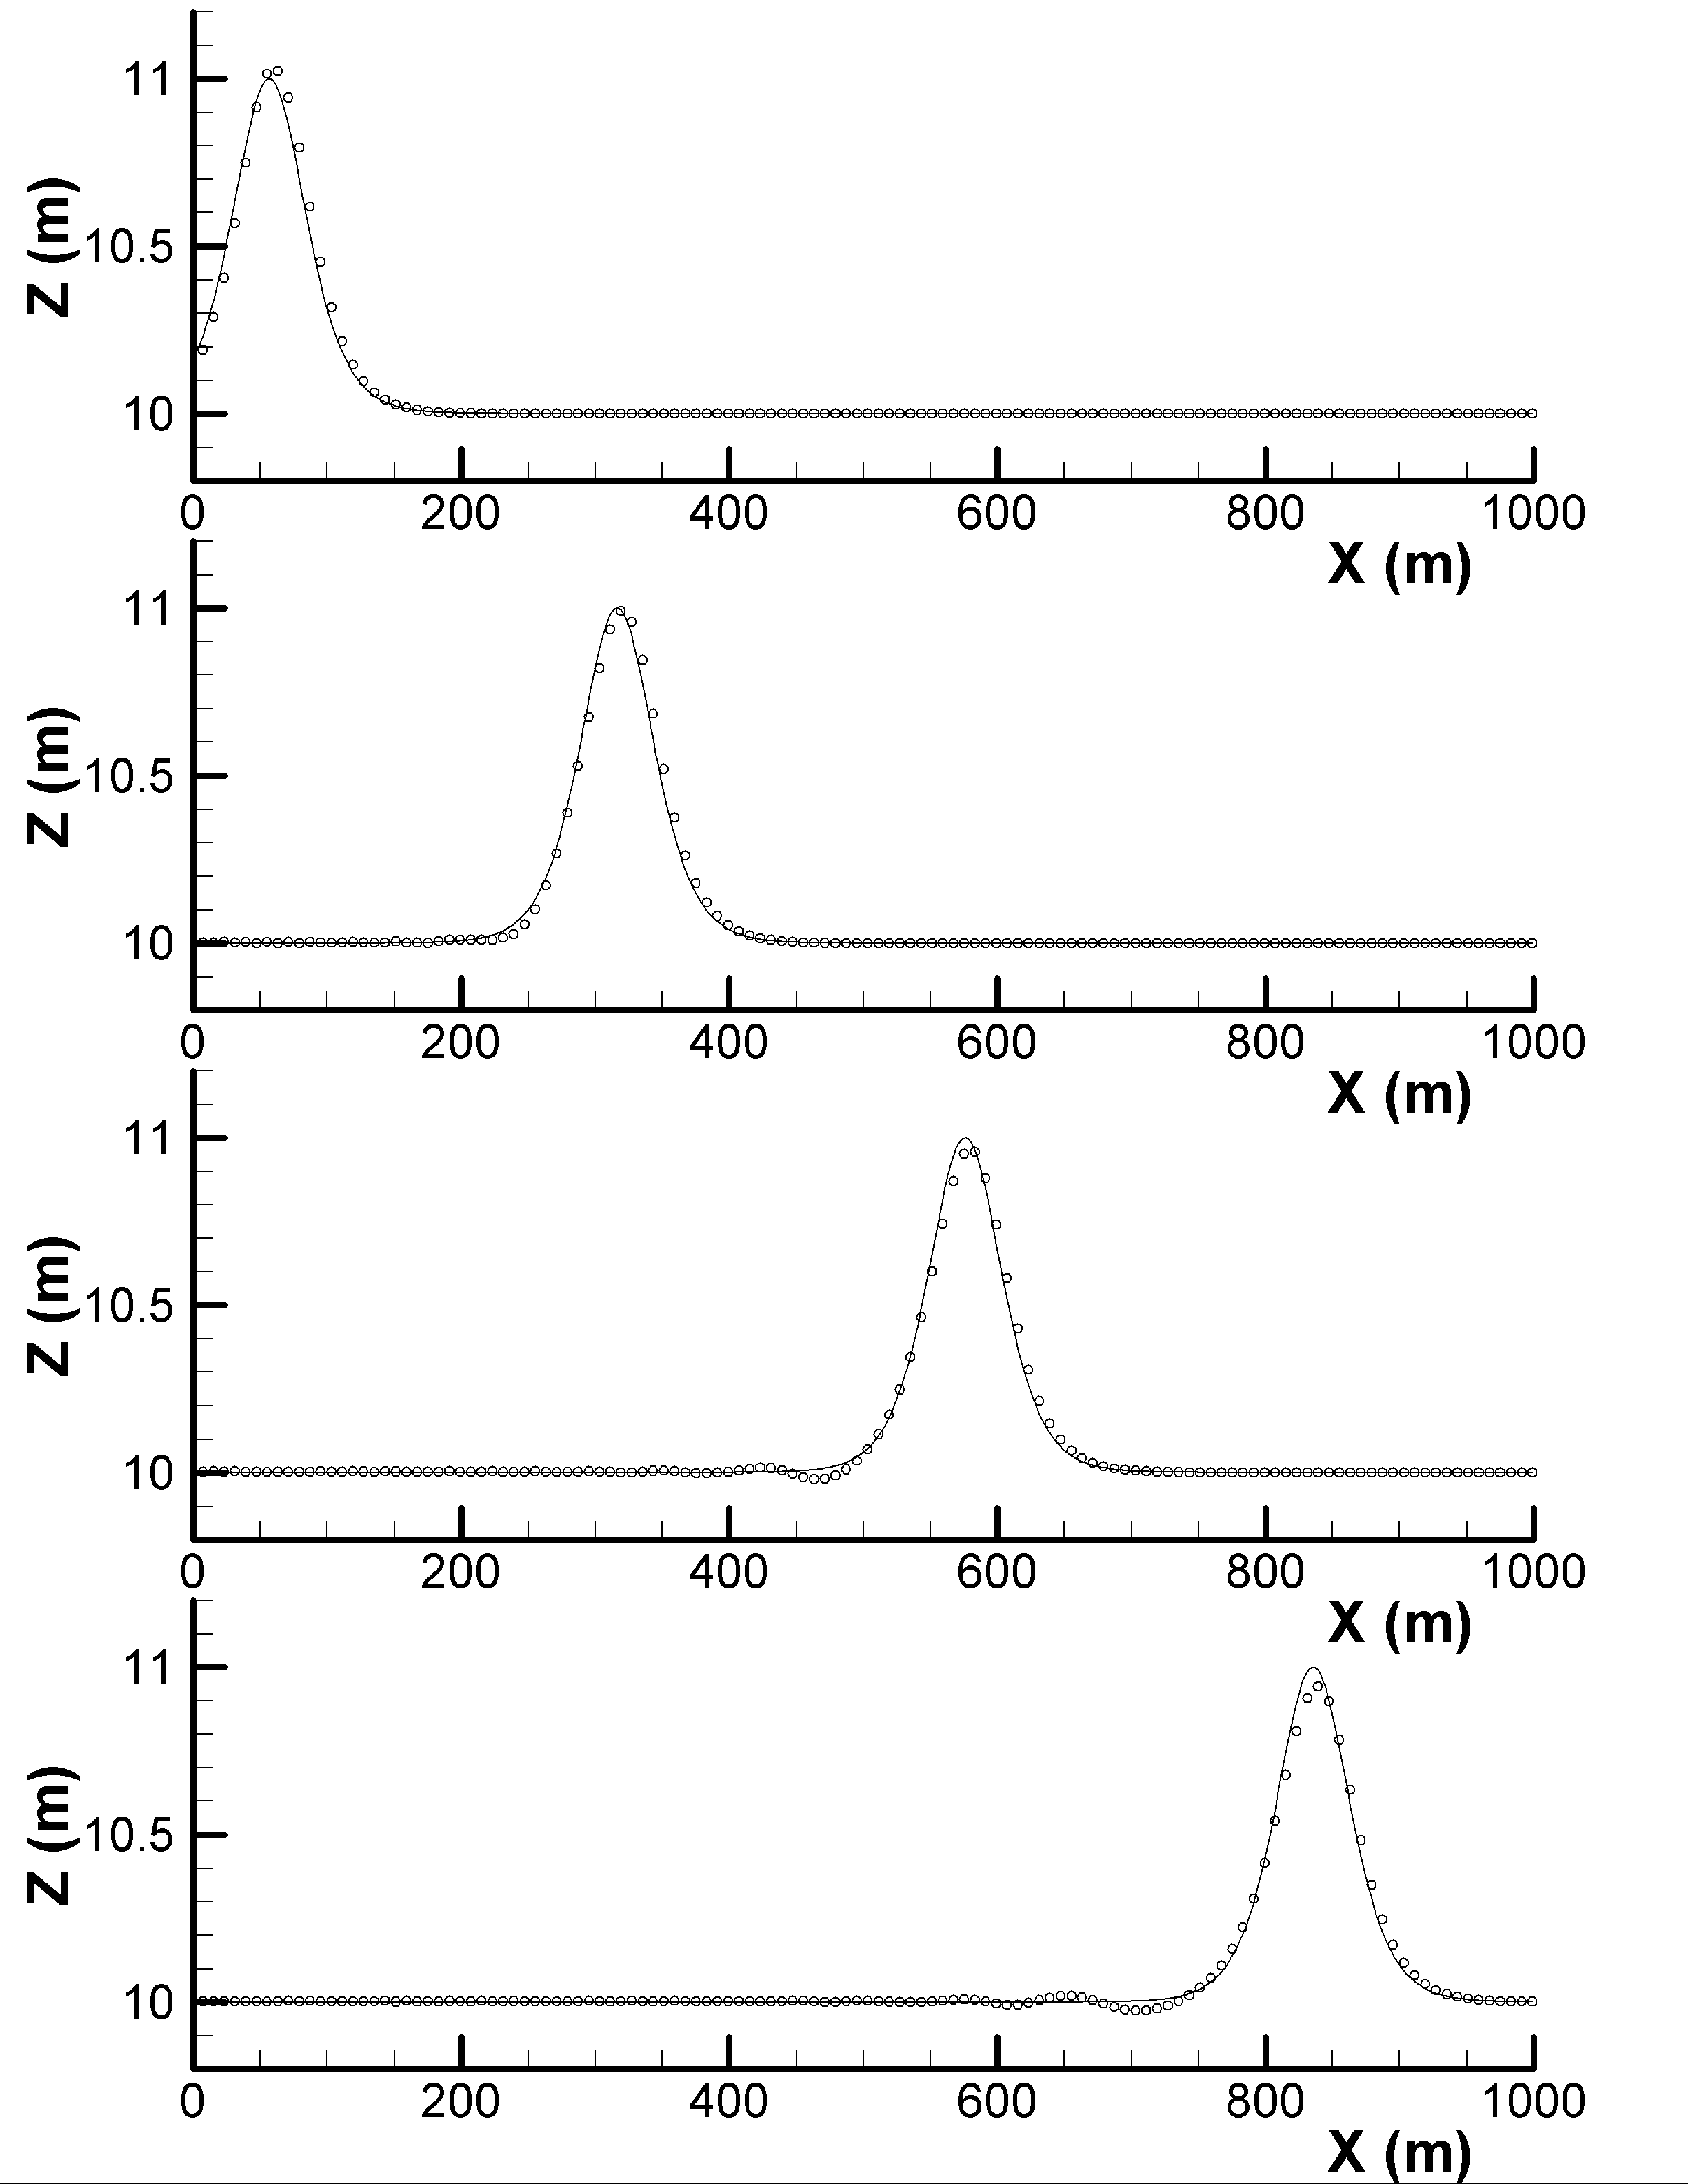
\includegraphics[width=4.5in]{../figures/SoliWav/SoliWav-LongCh-Ana-Num-Compar.pdf}
\label{fig:SoliWav-LongCh-Anal-Num-Compar}
\caption{Solitary wave test. Numerical solution versus analytical solution.}
\end{figure}

\cp
